\documentclass[12pt,a4paper]{article}
\usepackage{fullpage}
\usepackage[margin=2cm]{geometry}
\usepackage{amsmath}
\usepackage{subfig}
\usepackage{graphicx}
\usepackage[justification=centering]{caption}
\begin{document}
\title{Towards to automatic machine learning}
\author{LE Van Linh}
\date{August, 2018}
\maketitle
\begin{abstract}
In recent years, convolutional neural networks (CNNs) have been employed to many tasks of computer sciences, (i.e. images classification, object recognition, language modeling, \ldots) with many proposed networks: AlexNet, VGG, \ldots. Almost the networks are manually proposed and evaluated, which is time-consuming. Because of this, we are very interested in the methods of \textit{automating neural architecture search (NAS)}. In this study, we will provide an overview and the elements of neural architecture search. On that basis, we would like to apply the NAS to automatically propose the CNNs to predict the landmarks. By that, we can compare the results that obtained from automatic-model and manual-model (ICPRS-2018).
\end{abstract}

\section{Neural Architecture Search}

The successes of deep learning are remarkable by a lot of CNNs have been proposed in recent years. The networks, which have been designed from the simple to the complex, have helped the researchers solve the problems that we cannot finish before or we need a lot of time to provide the solution. However, most of CNNs are designed manually. In this period, NAS \cite{elsken2018neural} is known as a subfield of automated machine learning and it is considered as a solution to provide the neural architecture automatically. The NAS includes three components:
\begin{itemize}
	\item \textbf{Search space}: defines which architectures can be represented in principle.
	\item \textbf{Search strategy}: details how to explore the search space.
	\item \textbf{Performance estimation strategy}: refers to the process of estimating the performance of the architectures.
\end{itemize}
Fig.\ref{nas} shows the relation of the components in NAS.
\begin{figure}[h!]
	\centering
	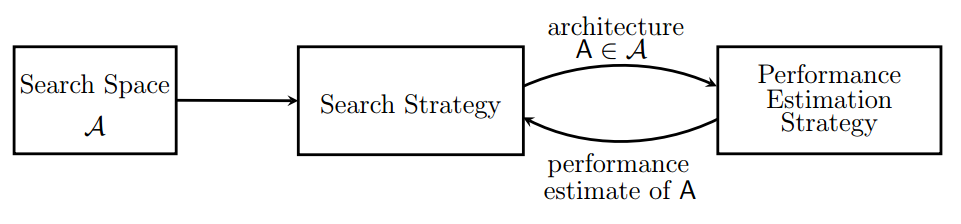
\includegraphics[scale=0.5]{images/nas/nas_components}
	\caption{Illustration of Neural Architecture Search method}
	\label{nas}
\end{figure}\\
The \textbf{Search space} contains almost the parameters of neural network. The \textbf{Search strategy} selects a network architecture $A$ from the search space. The selected network is passed to a \textbf{performance estimation strategy} to estimated the performances of network $A$ and return it to the search strategy. This process will be continued until reaching the stop conditions (i.e. how many trials?). For each performance time, the search strategy tries to modify the network A to obtain the best performance on the dataset.
\subsection*{Search space}
The search space defines which architectures can be represented in principle. For example to build a CNN, the search space is parameterized by:
\begin{itemize}
	\item The number of layers
	\item The type of layers (i.e. convolutional layer, pooling layer, full-connected layer, \ldots)
	\item The hyperparameters associated with the operations (i.e. CONV kernel, CONV filters, POOL kernel, \ldots)
\end{itemize}
The network hyperparameters are selected from the search space. They can be one-branch \cite{zoph2016neural, cai2018path} or multi-branch \cite{he2016deep, huang2017densely}, repeated motifs architectures \cite{zoph2017learning, szegedy2016rethinking, huang2017densely}.
Note that the difficulty of the optimization problem is depended on the size of the search space.
\subsection*{Search strategy}
Search strategy details the methods to explore the search space. It includes the algorithm to select a good parameters for an architecture after each step. Many different search strategies have been applied:
\begin{itemize}
	\item Random search
	\item Bayesian optimization
	\item Evolutionary methods
	\item Reinforcement learning (RL) \cite{sutton1998reinforcement} has been used in recent years
	\item Gradient-based methods
\end{itemize}
\subsection*{Performance estimation strategy}
Performance estimation strategy refers to the process of finding the architecture $A$ that maximizes the performance measure, such as accuracy, and reduce the cost of these performance estimation. The simplest way is to train $A$ on training data and to evaluate its performance on validation data. But training and evaluating A from scratch are time-consuming. So, to reduce the computation, some solutions have been proposed to get the better performance on this problem such as:
\begin{itemize}
	\item Shorter training times:
	\item Training on a subset of the data
	\item Training with less filters per layer
	\item Initialize the weight of next architecture based on the weights of other architectures that have been trained before (a kind of fine-tuning)
\end{itemize}

\section{Propose the solutions for landmarking networks}
Currently, \textit{most of the works on NAS are performed on images classification problem}. So, a strategy for a regression problem can be considered. Based on the knowledge about NAS, I would like to propose two strategies for detecting the landmarks on beetles.

In the first strategy, purpose is comparing the predicted landmarks which have obtained from a manual model (ICPRS-18) with the result of an automatic model. Firstly, a generic model has been designed with the same number of layers and the same type of the layers as the manual model. Then, the NAS will be applied to predict the hyperparameters for each layer in each trial during performance process. The model after each prediction will be trained and evaluated on the dataset. At the end of the process, we will compare the coordinates of the landmarks which have predicted by the manual and the automatic model.

In the second strategy, we will provide to NAS the number of layers and try to ask it the output of the network models. The models then are trained and evaluated on the dataset. Of course, at the end of the process, we also compare the results of the automatic models with the manual model.

In both of strategies, we use Reinforcement learning as a solution for the search strategy. Besides, all the proposed models will be trained from the scratch (before try with other solutions).
\bibliographystyle{unsrt}
\bibliography{includes/references}
\pagebreak

\end{document}